
\chapter{Justificación del proyecto}\label{cap:justificacion_proyecto}

%\subsection{Nueva tecnología no es sinónimo de mejores soluciones}
%TODO

A continuación se discutirán las razones para considerar el desarrollo de una plataforma \gloss{ecommerce}, un aporte en relación a las opciones \textit{open source} actualmente vigentes. Para esto se explicara por que los cambios de tecnología propuestos son un beneficio para el actual estado del arte del tema, asi como un aporte para potenciales funcionalidades que seran agregadas en el futuro.

\section{Base de datos}

\textit{Relational databases} se encuentran en la mayoría de las organización desde hace muchísimo tiempo, y por buenas razones. \textit{Relational databases} apoya las aplicaciones del pasado que cumplen con las necesidades de negocio actuales; Estas son apoyadas por un extenso ecosistema de herramientas; y hay una gran cantidad de mano de obra calificada para implementar y mantener estos sistemas.
%Relational databases have a long-standing position in most
%organizations, and for good reason. Relational databases
%underpin legacy applications that meet current business
%needs; they are supported by an extensive ecosystem of
%tools; and there is a large pool of labor qualified to
%implement and maintain these systems.

Pero las compañías están cada vez mas considerando la opción de alternativas para la infraestructura relacional heredada. En algunos casos la motivación es técnica, tal como la necesidad de escalar o actuar mas allá de las capacidades de sus sistemas actuales. Mientras que en otros casos, las compañías están motivadas por el deseo de identificar alternativas viables a \textit{softwares} propietario de alto costo. Una tercera motivación es la agilidad y velocidad del desarrollo, dado que las compañías ansían adaptarse al mercado mas rápido y adoptar metodologías de desarrollo ágil.
%But companies are increasingly considering alternatives to
%legacy relational infrastructure. In some cases the
%motivation is technical — such as a need to scale or
%perform beyond the capabilities of their existing systems —
%while in other cases companies are driven by the desire to
%identify viable alternatives to expensive proprietary
%software. A third motivation is agility or speed of
%development, as companies look to adapt to the market
%more quickly and embrace agile development
%methodologies.

Estas opciones se aplican tanto para aplicaciones analíticas como transaccionales. Las compañías están cambiando \textit{workloads to Hadoop} para sus \textit{offline}, \textit{analytical workloads}, y están construyendo \textit{online}, aplicaciones operaciones con una nueva clase de tecnología de manejo de datos llamada "\gloss{nosql}", como por ejemplo \textit{MongoDB}
%These drivers apply both to analytical and transactional
%applications. Companies are shifting workloads to Hadoop
%for their offline, analytical workloads, and they are building
%online, operational applications with a new class of data
%management technologies called "NoSQL", or "Not Only
%SQL", such as MongoDB

\subsection{\gloss{sql} and the Relational Model}

\gloss{sql} es un lenguaje declarativo de consulta de datos . Un lenguaje declarativo es uno en el cual un programador especifica lo que desea y el sistema lo ejecuta, en lugar de definir proceduralmente como el sistema debería hacerlo. Unos pocos ejemplos incluyen: encontrar el registro del empleado 39, mostrar solo el nombre y el numero de teléfono del empleado de la totalidad de su registro, filtrar los registros de los empleados a aquellos que trabajan en contabilidad, contar la cantidad de empleados en cada departamento, unir la información de la tabla de los empleados \textit{employees} con la tabla de \textit{managers}.
%SQL is a declarative language for querying data. A declarative language is one in which a programmer specifies what they want the system to do, rather than procedurally defining how the system should do it. A few examples include: find the record for employee 39, project out only the employee name and phone number from their entire record, filter employee records to those that work in accounting, count the employees in each department, or join the data from the employees table with the managers table.


En una primera aproximación, \gloss{sql} permite consultar sobre aquellas preguntas sin pensar sobre como la información es expuesta en el disco, cuales indices utilizar para acceder a la información o que algoritmo utilizar para procesar la información. Un componente arquitectural significativo para la mayoría de los \textit{relational databases is a query optimizer}, el cual decide cual de las muchos equivalentes lógicos planea ejecutar las respuesta mas rápida a una \textit{query}. Estos optimizadores son usualmente mejores que los promedios de los usuarios de la \textit{database}, pero en algunas ocasiones ellos no tienen la suficiente información o tienen un modelo muy simple del sistema en \textit{order} para generar ejecuciones mas eficientes.
%To a first approximation, SQL allows you to ask these questions without thinking about how the data is laid out on disk, which indices to use to access the data, or what algorithms to use to process the data. A significant architectural component of most relational databases is a query optimizer, which decides which of the many logically equivalent query plans to execute to most quickly answer a query. These optimizers are often better than the average database user, but sometimes they do not have enough information or have too simple a model of the system in order to generate the most efficient execution.

\textit{Relational databases}, las \textit{databases} mas utilizadas en la practica, siguen el modelo de datos relacional. En este modelo, diferentes entidades del \textit{real-world} son guardadas en diferentes tablas. Por ejemplo, todos los \textit{employees} podrían ser guardados en una tabla \textit{Employees}, y todos los \textit{departments} podrían ser almacenados en la tabla \textit{Departments}. Cada fila de una tabla tiene varias propiedades guardadas en columnas. Por ejemplo, \textit{employees} podrían tener un \textit{employee id}, \textit{salary}, \textit{birth date}, y \textit{first/last names}. Cada una de estas propiedades sera guardada en una columna de la tabla \textit{Employees}
%Relational databases, which are the most common databases used in practice, follow the relational data model. In this model, different real-world entities are stored in different tables. For example, all employees might be stored in an Employees table, and all departments might be stored in a Departments table. Each row of a table has various properties stored in columns. For example, employees might have an employee id, salary, birth date, and first/last names. Each of these properties will be stored in a column of the Employees table.


El modelo relacional, va mano a mano con \gloss{sql}. \textit{Queries} simples de \gloss{sql}, tales como filtrar, recuperar todos los registros el cual sus campos hagan \textit{match} en algunos test (ejemplo, \textit{employeeid} = 3, o salary > \$ 20000). Constructores mas complejos causan que \textit{database} haga trabajo extra, tal como \textit{joining} información sobre múltiples tablas (ejemplo., ¿ Cuál es el nombre del departamento en donde \textit{employee} 3 trabaja?). Otras estructuras complejas tal como \textit{aggregates} (ejemplo, ¿ cuál es el salario promedio de mis empleados?) puede manejar para \textit{full-table scans}.
%The relational model goes hand-in-hand with SQL. Simple SQL queries, such as filters, retrieve all records whose field matches some test (e.g., employeeid
% = 3, or salary \> \$ 20000). More complex constructs cause the database to do some extra work, such as joining data from multiple tables (e.g., what is the name of the department in which employee 3 works?). Other complex constructs such as aggregates (e.g., what is the average salary of my employees?) can lead to full-table scans.


\textit{Relational data model} define entidades altamente estructuradas con relaciones estrictas entre ellos. \textit{Querying} este modelo con \gloss{sql} permite \textit{complex data transversa} sin desarrollar mucho. La complejidad del modelo y \textit{quering}, tienen sus limites, aunque:
%The relational data model defines highly structured entities with strict relationships between them. Querying this model with SQL allows complex data traversals without too much custom development. The complexity of such modeling and querying has its limits, though:

\textit{Complexity} guia a \textit{unpredictability}. La expresivilidad en \gloss{sql} implica un desafío en relación al costo de cada \textit{query}, y así el costo de \textit{workload}. Mientras, lenguajes de \textit{query} simples pueden complicar la lógica, al mismo tiempo hacen que sea sencillo proveer de almacenamiento de datos., cuando solo responde a \textit{requests} simples.
%Complexity leads to unpredictability. SQL's expressiveness makes it challenging to reason about the cost of each query, and thus the cost of a workload. While simpler query languages might complicate application logic, they make it easier to provision data storage systems, which only respond to simple requests.

Hay muchas maneras de modelar un problema. \textit{Relational data model} es estricto: El \textit{schema} asignado para cada tabla especificada la \textit{data} en cada fila. Si se esta almacenando menos \textit{data} estructurada, o filas con mas diferencia en las columnas que se guardan, \textit{relational model} puede ser innecesariamente restrictiva. Similarmente, aplicaciones desarrolladas podrían no encontrar el \textit{relational model} idóneo para modelar cada tipo de \textit{data}. Por ejemplo, una gran cantidad den aplicaciones lógicas son escritas en lenguaje \textit{object-oriented} e incluye conceptos \textit{high-level} tales como \textit{lists}, \textit{queues}, y \textit{sets}, y algunos programadores desearan \textit{persistence layer} para modelar esto.
%There are many ways to model a problem. The relational data model is strict: the schema assigned to each table specifies the data in each row. If we are storing less structured data, or rows with more variance in the columns they store, the relational model may be needlessly restrictive. Similarly, application developers might not find the relational model perfect for modeling every kind of data. For example, a lot of application logic is written in object-oriented languages and includes high-level concepts such as lists, queues, and sets, and some programmers would like their persistence layer to model this.

Si la \textit{data} crece mas allá de la capacidad de un servidor, entonces las tablas en la \textit{database} tendrá que ser particionado a través de varios computadores. Para evitar \textit{JOINs} a través de la red para obtener todas las tablas requeridas, será necesario desnormalizarla. Desnormalizar consiste en guardar toda la \textit{data} de diferentes tablas que se desean consultar en el mismo lugar. Esto hace que la \textit{database} simule una \textit{key-lookup store system}, dejando preguntas sobre la posibilidad de adaptarse mejor a la \textit{data}.
%If the data grows past the capacity of one server, then the tables in the database will have to be partitioned across computers. To avoid JOINs having to cross the network in order to get data in different tables, we will have to denormalize it. Denormalization stores all of the data from different tables that one might want to look up at once in a single place. This makes our database look like a key-lookup storage system, leaving us wondering what other data models might better suit the data.

Generalmente no es inteligente descartar años de consideraciones de diseño arbitrariamente. Cuando se considera el almacenamiento de la \textit{data} en una \textit{database}, considera \gloss{sql} y \textit{relational model}, los cuales son respaldados por décadas  de investigación y desarrollo, ofreciendo enriquecidas capacidades de modelamiento, y proveer garantías \textit{fácil-de-entender} sobre operaciones complejas. \gloss{nosql} es una buena opción cuando se tiene un problema específico, tal como gran cantidad de \textit{data}, un masivo \textit{workload}, o una difícil decisión de modelamiento para la cual \gloss{sql} y \textit{relational databases} podrían no haber sido optimizadas.
%It's generally not wise to discard many years of design considerations arbitrarily. When you consider storing your data in a database, consider SQL and the relational model, which are backed by decades of research and development, offer rich modeling capabilities, and provide easy-to-understand guarantees about complex operations. NoSQL is a good option when you have a specific problem, such as large amounts of data, a massive workload, or a difficult data modeling decision for which SQL and relational databases might not have been optimized.

\subsection{NoSQL}

\gloss{nosql} engloba una gran variedad de diferentes \textit{database technologies} y fueron desarrolladas en respuesta al creciente volumen de \textit{data} guardada de los usuarios, objetos y productos, la frecuencia en que la \textit{data} es accesada, y la \textit{performance} en las necesidades de los procesos. \textit{Relational database}, por otra parte, no fueron diseñadas para hacer frente a los desafíos de escalabilidad y agilidad que enfrentan las aplicaciones modernas, no fueron construidas para tomar ventaja del almacenamiento barato y el poder de procesamiento disponible en la actualidad.
%NoSQL encompasses a wide variety of different database technologies and were developed in response to a rise in the volume of data stored about users, objects and products, the frequency in which this data is accessed, and performance and processing needs. Relational databases, on the other hand, were not designed to cope with the scale and agility challenges that face modern applications, nor were they built to take advantage of the cheap storage and processing power available today.

\subsubsection{Document Model}\label{cap:justificacion_proyecto:tecnologias:nosql:document_model}
 Mientras \textit{relational databases store data} en filas y columnas, \textit{document databases store data} en documentos.  

Estos documentos tipicamente usan una estructura equivalente a \gloss{json}, un formato muy popular entre desarrolladores. \textit{Documents} proveen una manera intuitiva y natural para modelar \textit{data} que esta cercanamente alineada con  programación \textit{object-oriented}, en el cual cada documento es efectivamente un objeto. Los documentos contienen uno o mas campos, donde cada campo contiene un tipo de valor, tales como \textit{string}, \textit{date}, \textit{binary}, o \textit{array}. En lugar de extenderse un registro entre múltiples tablas y columnas, cada registro y su \textit{data} asociada son tipicamente almacenadas juntas en un solo documento. Esto simplifica el acceso a la \textit{data} y reduce e incluso elimina la necesidad de \textit{joins} y\textit{complex transactions}.

En un \textit{document database}, la noción de esquema es dinámica: cada documento puede contener diferentes campos. Esta flexibilidad puede ser particularmente útil para modelar \textit{data} sin estructura y \textit{polymorphic}. Esto también hace posible la evolución de una aplicación durante su desarrollo, simplemente agregando nuevos campos. Adicionalmente, \textit{document databases} generalmente proveen consultas robustas que los desarrolladores esperan en \textit{relational databases}.

Aplicaciones:\textit{Document databases} son de propósito general y útiles para una amplia variedad de aplicaciones, debido a su flexibilidad del \textit{data model}, la habilidad para consultar sobre cualquier campo y el \textit{natural mapping} del \textit{document data model} a objetos en programación de lenguajes modernos.

Ejemplos: MongoDB y CouchDB.

\subsubsection{Graph Model}

Basado en \nameref{ap:apendice_B}, usa estructuras de grafos con nodos, bordes y propiedades para representar la \textit{data}. En esencia, la \textit{data} es modelada como una red de relaciones entre elementos específicos. Si bien es cierto, \textit{Model Graph}, puede ser contra intuitivo y tomar tiempo para entenderlo, puede ser utilizado extensamente para numerosas aplicaciones. Su principal característica es que modela fácilmente las relaciones entre entidades en una aplicación.

Aplicaciones:\textit{Graph databases} son útiles en escenarios donde las relaciones son el \textit{core} de la aplicación, como redes sociales.

Ejemplos: Neo4j y HyperGraphDB.

\subsubsection{Key-Value}

Desde una perspectiva de\textit{data model}, \textit{key-value stores} son el tipo mas básico de las \textit{\gloss{nosql} databases}. Cada \textit{item} en la \textit{database} es guardado como un atributo \textit{name}, ó \textit{key}, junto con su \textit{value}. El \textit{value}, sin embargo, es totalmente \textit{opaque} al sistema;la \textit{data} solo puede ser requerida desde la \textit{key}. Este modelo puede ser útil para \textit{representig polymorphic} y \textit{unstructured data}, dado que la \textit{database} no define un \textit{scheme} al conjunto \textit{key-value}.
%From a data model perspective, key-value stores are the most basic type of NoSQL database. Every item in the database is stored as an attribute name, or key, together with its value. The value, however, is entirely opaque to the system; data can only be queried by the key. This model can be useful for representing polymorphic and unstructured data, as the database does not enforce a set schema across key-value pairs.

\subsubsection{Wide Column Models}

%Wide column stores, or column family stores, use a sparse,
%distributed multi-dimensional sorted map to store data. Each record can vary in the number of columns that are stored, and columns can be nested inside other columns called super columns. Columns can be grouped together for access in column families, or columns can be spread across multiple column families. Data is retrieved by primary key per column family.
%
%Applications: Key value stores and wide column stores are useful for a narrow set of applications that only query data by a single key value. The appeal of these systems is their performance and scalability, which can be highly optimized due to the simplicity of the data access patterns.
%
%2Examples: Riak and Redis (Key-Value); HBase and Cassandra (Wide Column).





\begin{table}[h!]
    \tiny
   
%\begin{tabular}{ |C{0.3\paperwidth}|C{0.3\paperwidth}| }
\begin{tabular}{ |L{0.1\paperwidth}|L{0.3\paperwidth}|L{0.3\paperwidth}|}
\hline
	&
	SQL Databases &
	NoSQL Databases
 
\\ \hline
	Types&
	One type (SQL database) with minor variations&
	Many different types including key-value stores, document databases, wide-column stores, and graph databases
	
\\ \hline
	Development History&
	Developed in 1970s to deal with first wave of data storage applications&
	Developed in 2000s to deal with limitations of SQL databases, particularly concerning scale, replication and unstructured data storage
	
\\ \hline
	Examples&
	MySQL, Postgres, Oracle Database&
	MongoDB, Cassandra, HBase, Neo4j
\\ \hline
	Data Storage Model&
	Individual records (e.g., "employees") are stored as rows in tables, with each column storing a specific piece of data about that record (e.g., "manager," "date hired," etc.), much like a spreadsheet. Separate data types are stored in separate tables, and then joined together when more complex queries are executed. For example, "offices" might be stored in one table, and "employees" in another. When a user wants to find the work address of an employee, the database engine joins the "employee" and "office" tables together to get all the information necessary.&
	Varies based on database type. For example, key-value stores function similarly to SQL databases, but have only two columns ("key" and "value"), with more complex information sometimes stored within the "value" columns. Document databases do away with the table-and-row model altogether, storing all relevant data together in single "document" in JSON, XML, or another format, which can nest values hierarchically.
	

\\ \hline
	Schemas&
	Structure and data types are fixed in advance. To store information about a new data item, the entire database must be altered, during which time the database must be taken offline.&
	Typically dynamic. Records can add new information on the fly, and unlike SQL table rows, dissimilar data can be stored together as necessary. For some databases (e.g., wide-column stores), it is somewhat more challenging to add new fields dynamically.

\\ \hline
	Scaling&
	Vertically, meaning a single server must be made increasingly powerful in order to deal with increased demand. It is possible to spread SQL databases over many servers, but significant additional engineering is generally required.&
	Horizontally, meaning that to add capacity, a database administrator can simply add more commodity servers or cloud instances. The database automatically spreads data across servers as necessary.
	
\\ \hline
	Development Model&
	Mix of open-source (e.g., Postgres, MySQL) and closed source (e.g., Oracle Database)&
	Open-source
	
\\ \hline
	Supports Transactions&
	Yes, updates can be configured to complete entirely or not at all&
	In certain circumstances and at certain levels (e.g., document level vs. database level)
	
\\ \hline
	Data Manipulation&
	Specific language using Select, Insert, and Update statements, e.g. SELECT fields FROM table WHERE…&
	Through object-oriented APIs

\\ \hline
	Consistency&
	Can be configured for strong consistency&
	Depends on product. Some provide strong consistency (e.g., MongoDB) whereas others offer eventual consistency (e.g., Cassandra)

\\ \hline
\end{tabular}
    \caption{ Resumen NoSQL vs. SQL}
    \label{tab:SQL_vs_noSQL_summary}
\end{table}

\subsection{MongoDB y E-Commerce \cite{online_mongodb_ecommerce}}
\label{cap:justificacion_proyecto:MongoDB_ECommerce}

Demostración de \textit{next-generation data stores} tipicamente giran en torno a \textit{social network}: Twitter, Facebook, Foursquare, etc. Desafortunadamente, tales aplicaciones tienden a tener complejos \textit{data models}. \textit{E-Commerce} por ejemplo, tiene la ventaja de incluir un largo número de patrones familiares para \textit{data modeling}. Ademas no es complicado imaginar como \textit{products, categories, product reviews} y \textit{orders} son típicamente modeladas en \gloss{rdbms}.

\textit{E-Commerce} han sido usualmente un dominio exclusivo de \gloss{rdbms}s, y esto es así por un par de razones. La primera, es que \textit{\gloss{ecommerce} sites} generalmente requieren \textit{transactions}, y \textit{transactions} son una operación básica en \gloss{rdbms}. Lo segundo es que, hasta hace poco, dominios que requieren de un \textit{rich data model} y sofisticadas \textit{queries} ha sido presupuesto que se ajustan mejor en \gloss{rdbms}. En las siguientes secciones se cuestionara la segunda afirmación. 

\subsubsection{\textit{Catalog Management}}

Si es necesaria información sobre como el \textit{catalog management} se maneja con \textit{relational databases}, es necesario dar una mirada rápida a los \textit{schemas} del popular Magento \textit{e-Commerce framework} \ref{ap:figure:catalog_magento} o OfBiz de Apache \ref{ap:figure:catalog_ofbiz}. Lo que se observa es un conjunto de tablas trabajando a la par para proveer un \textit{schema} flexible sobre un fundamentalmente inflexible estilo de \textit{database system}.

Esto significa que la \textit{data} de cualquier producto se extiende a través de una docena de tablas. Esto incremente la complejidad del código requerido para la persistencia de consultas de productos individuales y hacer una consulta \textit{shell-based} es casi imposible. Simplemente considere escribir un \gloss{sql} JOIN para para reunir el modelo de un producto como esto:

\begin{figure}[h!]
	\centering
	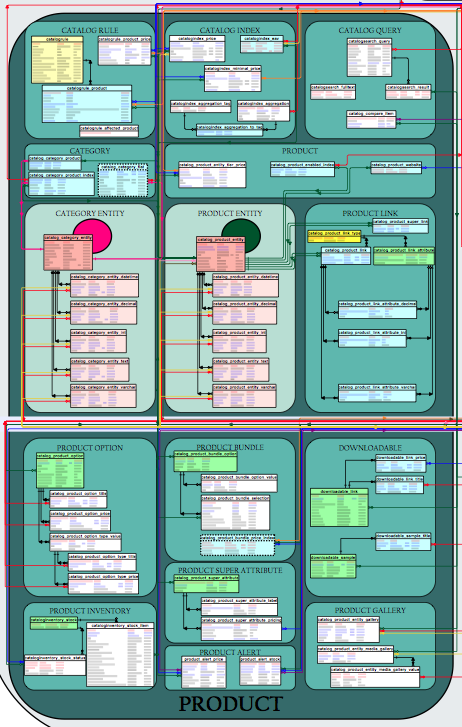
\includegraphics[width=0.3\textwidth]{figuras/cap2/magento_product_schema.png}
	\caption{\textit{Schemas}de un producto.}
	\label{cap:figure:catalog_magento}
\end{figure}

O realizar una sencilla búsqueda desde MongoDB JavaScript \textit{shell} para obtener un objecto \gloss{json} como este:

\medskip
\begin{lstlisting}[caption= Busqueda en MongoDB]

db.products.find({'_id': ObjectID("4bd87bd8277d094c458d2fa5")});

{_id: ObjectID("4bd87bd8277d094c458d2a43"),
 title: "A Love Supreme [Original Recording Reissued]"
 author: "John Coltrane",
 author_id: ObjectID("4bd87bd8277d094c458d2fa5"),

 details: {
   number_of_discs: 1,
   label: "Impulse Records",
   issue_date: "December 9, 1964",
   average_customer_review: 4.95,
   asin: "B0000A118M"
 },

 pricing: {
  list: 1198,
  retail: 1099,
  savings: 99,
  pct_savings: 8
 },

 categories: [
   ObjectID("4bd87bd8277d094c458d2a43"),
   ObjectID("4bd87bd8277d094c458d2b44"),
   ObjectID("4bd87bd8277d094c458d29a1")
 ]
}
\end{lstlisting}

Claramente no es una representación completa de un producto, pero esto demuestra cuantas de estas tablas triviales que existen en una \textit{relational representation} pueden prescindir en un \textit{document representation}.

Para \textit{object-oriented data}, los documentos tienen mayor sentido, tanto en concepto como rendimiento. Una representación \textit{document-oriented} de una \textit{data} de un producto se traduce a unas pocas entidades (un puñado de \textit{collections} vs. una docena de tablas), mejor \textit{performance} en consultas (sin \textit{sever-side joins}), y estructuras que corresponden precisamente al producto. Ya no existe la necesidad de diseñar un \textit{master schema} que pueda considerar a cada tipo de producto concebible.

\textit{Catalog management} es esencialmente \textit{content management}, un campo en donde MongoDB sobresale.

\subsubsection{Shopping Carts and Orders}

Permitir que un \textit{shopping cart} sea simplemente una orden en un estado del \textit{\"cart\"}, el modelo de \textit{shopping carts} y las ordenes en MongoDB se tornan muy sencillas:

\medskip
\begin{lstlisting}[caption= Estructura de una orden.]

{'_id': objectid('4b980a6dea2c3f4579da141e'),
 'user_id': objectid('4b980a6dea2c3f4579a4f54'),
 'state': 'cart',

 'line_items': [
    {'sku': 'jc-432',
     'name': 'John Coltrane: A Love Supreme',
     'retail_price': 1099
    },

    {'sku': 'ly-211',
     'name': 'Larry Young: Unity',
     'retail_price': 1199
    },
  ],

 'shipping_address': {
   'street': '3333 Greene Ave.',
   'city': 'Brooklyn',
   'state': 'NY',
   'zip': '11216'
  },

  'subtotal': 2199
}
\end{lstlisting}

Notar que es posible presentar los pedidos como un \textit{array} de productos. Como es usual con documentos, esto hace el despliegue del \textit{shopping cart} mas sencillo, dado que no hay \textit{joins} envueltos. Pero esto también resuelve el problema del versionamiento de productos. Usualmente es necesario tener el estado de un producto cuando este es comprado. Esto puede ser logrado en una \gloss{rdbms} estableciendo un vinculo a versiones particulares de un producto. Aquí, sin embargo, simplemente se almaceno el estado de un producto dentro de la misma orden.

\subsubsection{\textit{Querying Orders}}

Dado que MongoDB soporta consultas dinámicas y \textit{secondary indexes}, las consultas para las ordenes son automáticas. Es posible, por ejemplo, definir un \textit{index} en un \textit{product \gloss{sku}}, lo que permite consultas eficientes en todas las ordenes para un producto dado:

\medskip
\begin{lstlisting}[caption= Consulta eficiente con \textit{secondary indexes}.]
	db.orders.ensureIndex({'line_items.sku': 1});
	db.orders.find({'line_items.sku' => 'jc-431'});
\end{lstlisting}

Con MongoDB, es posible realizar consultas en atributos arbitrarios, de esa manera cualquier \textit{query}, en \textit{orders collection} es posible. Y para \textit{queries} comunes, es posible definir \textit{indexes} para una mejor eficiencia.

\subsubsection{\textit{Aggregation}}

Claramente, \textit{aggregation} también es necesario. Se desea reportar ordenes de diferentes maneras, y para ese propósito, \textit{map-reduce} esta disponible. Como ejemplo, el comando \textit{map-reduce} que \textit{aggregtes} el total de ordenes por \textit{zip code}:

\begin{lstlisting}[caption= Ejemplo de commando \textit{map-reduce}.]
map = "
  function() {
    emit(this['shipping_address']['zip'], {total: this.total})
  }"

reduce = "
  function(key, values) {
    var sum = 0;
    values.forEach(function(doc) {
      sum += doc.total;
    }

    return {total: sum};
  }"


db.orders.mapReduce(map, reduce, {out: 'order_totals_by_zip'});
\end{lstlisting}

\subsubsection{Updating Orders}

\subsubsection*{Incrementing Quality}

Una manera de ajustar la cantidad es usando un \textit{position operator}, el cual permite aplicar \textit{atomic operations}, a un único objeto dentro de un \textit{array}. A continuación se muestra como cambiar el numero de álbumes que se están ordenando:

\begin{lstlisting}[caption= Ejemplo de \textit{atomic operation}.]
	db.orders.update({'_id': order_id, 'line_items.sku':'jc-431'},
		{'$set': {'line_items.$.quantity': 2}});
\end{lstlisting}

 
\subsubsection*{Adding and Removing Items}

Igualmente, \textit{atomic operators} resuelven el problema de agregar y remover productos desde el carro. Por ejemplo, se puede utilizar \$push \textit{atomic operator} para agregar un item al \textit{cart};

\begin{lstlisting}[caption= Ejemplo de \textit{atomic operation}.]
	db.orders.update({'_id': order_id},
    {'$push': {'line_items':
      {'sku': 'md-12', 'price': 2500, 'title': 'Basketball'}}
     '$inc': {'subtotal': 2500}});
\end{lstlisting}

Al ajustar la cantidad y el cambio de los mismos \textit{items} en el \textit{cart}, es necesario actualizar el total de la orden. Notar el uso de \$inc \textit{operator} para manejar esto.

\subsubsection{Inventory}

No todos los sitios \textit{e-Commerce} necesitan manejar el inventario. Pero para aquellos que si lo hacen, MongoDB funciona a la altura de las circunstancias.

Una manera para manejar el inventario, es \textit{store} un documento separado por cada \textit{physical item} en la bodega. Así, por ejemplo, si la bodega tiene veinte copias del álbum Coltrane, se traduce en veinte documentos distintos en \textit{inventory collection}. Cada documento tiene una estructura como la siguiente:

\begin{lstlisting}[caption= Ejemplo de \textit{atomic operation}.]
	{'_id': objectid('4b980a6dea2c3f4579da432a'),
 'sku': 'jc-431',
 'state': 'available',
 'expires': null,
 'order_id': null
}
\end{lstlisting}


Cuando un usuario intenta agregar un \textit{item} al \textit{cart}, un \textit{findAndModify command} puede ser facilitado para \textit{atomically mark} el \textit{item} en \textit{in-cart}, asociando el \textit{item} con una orden dada, y estableciendo un tiempo de expiración:

\begin{lstlisting}[caption= Ejemplo de \textit{atomic operation}.]
	query = {'sku': 'jc-431', 'state': 'available'};

update = {'$set':
          {'state':    'cart',
           'order_id': order_id,
           'expires':  Date.now() + 15 * 60}};

item = db.inventory.findAndModify(query: query, update: update);
\end{lstlisting}

Si se obtiene un \textit{item back} desde el \textit{findAndModify operation}, se sabe que tenemos un único \textit{lock} en el \textit{item}, y es posible \textit{store it} en el \textit{cart}. Cuando el usuario desea \textit{check out}, el estado del \textit{item} puede cambiar a \textit{"purchased"}, o cualquiera sea el caso de la llamada.

Mientras, se pueda ejecutar un \textit{script in the background} que libere el inventario del \textit{cart} que no ha sido \textit{purchased} en la ventana de quince minutos. La actualización es trivial:

\begin{lstlisting}[caption= Ejemplo de \textit{atomic operation}.]
	db.inventory.update({'state': 'cart', 'expires': {'$lt': Date.now()}},
  {'$set' {'state': 'available', 'expires': null, 'order_id': null}},
  {multi: true});
\end{lstlisting} 

\subsubsection{\textit{Transactions}, \textit{Consistency} y \textit{Durability}}

Muchos argumentos impuestos contra NoSQL en \textit{e-Commerce} se centran en \textit{transactions}, \textit{consistency}, y \textit{durability}. En relación a esto se mencionan algunos puntos.

En relación a \textit{transactions}, ciertamente MongoDB no soporta el tipo \textit{multi-object}; sin embargo, soporta \textit{atomic operations} sobre documentos individuales. y esto combinado con \textit{documento-oriented modeling} recién descrito y creatividad, es suficiente para muchos problemas \textit{e-Commerce}. Ciertamente, si se necesita \textit{debit one account} y \textit{credit another} en la misma operación, o si se desea \textit{rollback}, sera necesario \textit{full-fledged transactions}. No obstante, \textit{transactionality} provista por MongodB debería ser suficiente en la mayoría de los casos, si no en todos, para \textit{e-Commerce operations}.

Si la preocupación esta sobre \textit{consistency} y \textit{durability}, operaciones escritas en MongoDB pueden ser realizadas \textit{consistency} sobre conexiones. Ademas, MongoDB 1.5 soporta \textit{near-real-time replications}, así que es posible asegurarse que una operación ha sido \textit{replicated} antes de retornar.

\subsubsection{\textit{Scalability}}
La manera mas sencilla para \textit{scale} la mayoría de las \textit{databases}, es \textit{upgrading} el \textit{hardware}. Si la aplicación esta corriendo en un único nodo, es usualmente posible agregar una combinación de \textit{disk} IOPS, \textit{memory}, y CPU para eliminar los cuello de botella de la \textit{database}.La técnica de mejorar el \textit{hardware} de un solo node para escalar se conoce como \textit{vertical scaling} o \textit{scaling up}. \textit{Vertical scaling} tiene la ventaja de ser simple, seguro, y \textit{cost-effective} hasta un cierto punto. Si se esta ejecutando sobre un \textit{virtualized hardware}( tal como \textit{Amazon's EC2}), entonces puedes encontrar que una instancia lo suficientemente larga no esta disponible. Si estas ejecutando sobre \textit{physical hardware}, habrá un punto donde el costo de un servidor mas poderoso se vuelve prohibitivo.

\begin{figure}[h!]
	\centering
	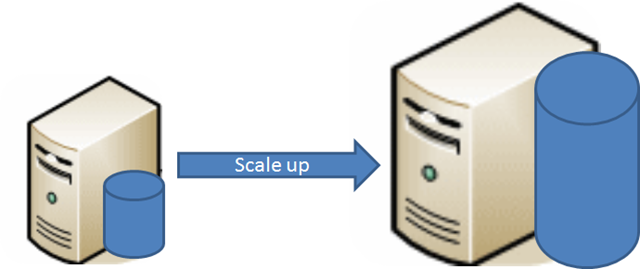
\includegraphics[width=0.5\textwidth]{figuras/cap2/scale_up.png}
	\caption{\textit{Vertical scaling} o \textit{Scaling up} }
\end{figure}

Entonces tiene sentido  considerar \textit{scaling horizontally} o \textit{scaling out}. En lugar de reforzar un único nodo, \textit{scalling horizontally} significa distribuir de \textit{database} sobre múltiples maquinas. Dado que \textit{horizontally scaled architecture} puede utilizar \textit{comodity hardware}, el costo de \textit{hosting} el total de la \textit{data} puede ser reducido significativamente. Incluso, la distribución  de \textit{data} sobre maquinas mitiga las consecuencias de fallo. Las maquinas inevitablemente fallaran de algún momento a otro. Si se \textit{scaled vertically} , y la maquina falla, entonces es necesario tratar con una falla en un maquina de la cual la mayoría del sistema depende. Podría no considerarse un tema si una copia de la \textit{data} existe en un \textit{replicated slave}, pero aun esta el caso e que solo un único \textit{sever} es necesario para bajar el sistema completo. En contraste con el fallo dentro de un \textit{horizontally scaled architecture}. Esto podría ser menos catastrófico dado que una sola máquina representa un porcentaje menor del sistema completo.

\begin{figure}[h!]
	\centering
	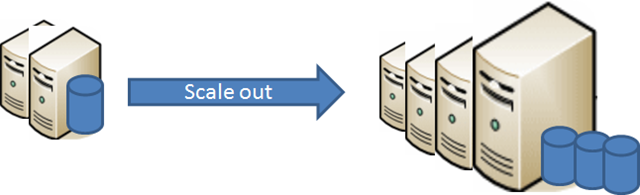
\includegraphics[width=0.5\textwidth]{figuras/cap2/scale_out.png}
	\caption{\textit{Horizontally scaling} o \textit{Scaling out} }
\end{figure}

MongoDB es un \textit{database management system} diseñado para hacer \textit{horizontal scaling} manejable, dado que fue construido para aplicaciones \textit{web} e infraestructuras de Internet.

\subsubsection{Conclusion}

Es cierto que la mayoría de \textit{NoSQL databases} no fueron construidas considerando \textit{e-Commmerce}. \textit{Databases} que carecen \textit{data models} enriquecidos, \textit{dynamic queries}, y la noción de \textit{transactionality} no puede esperarse que compitan en el espacio de \textit{e-Commerce}, entonces no es comprensible que no se considere MongoDB tampoco.

Pero para las partes en donde el sitio \textit{\gloss{ecommerce}} comprende el manejo de contenido, MongoDB es claro vencedor. E incluso para mas \textit{transactional components} del sistema, MongoDB tiene características que hacen de la posibilidad de correr un sistema completo de \textit{e-Commerce} una realidad.


\section{Node.js}

%La craciente popularidad de JavaScript a traiado consigo una gran cantidad de cambios, y la manera en la cual los desarrolladores afrontan el desarrollo \textit{web} es dramaticamente distinto. Las cosas que se pueden hacer en la \textit{web} estos dias con JavaScript Corriendo en el servidor, de la misma manera como en el browser, era dificilmente imaginable hasta hace unos años atras, o fuimos encaptulados dentro de ambientes de \textit{sandbox} como Flash o Java Applets.
%JavaScript’s rising popularity has brought with it a lot of changes, and the face of web development today is dramatically different. The things that we can do on the web nowadays with JavaScript running on the server, as well as in the browser, were hard to imagine just several years ago, or were encapsulated within sandboxed environments like Flash or Java Applets.

%Before digging into Node.js, you might want to read up on the benefits of using JavaScript across the stack which unifies the language and data format (JSON), allowing you to optimally reuse developer resources. As this is more a benefit of JavaScript than Node.js specifically, we won’t discuss it much here. But it’s a key advantage to incorporating Node in your stack.

%As Wikipedia states: “Node.js is a packaged compilation of Google’s V8 JavaScript engine, the libuv platform abstraction layer, and a core library, which is itself primarily written in JavaScript.” Beyond that, it’s worth noting that Ryan Dahl, the creator of Node.js, was aiming to create real-time websites with push capability, “inspired by applications like Gmail”. In Node.js, he gave developers a tool for working in the non-blocking, event-driven I/O paradigm.

%After over 20 years of stateless-web based on the stateless request-response paradigm, we finally have web applications with real-time, two-way connections.

En una frase: Node.js brilla en aplicaciones \textit{web} \textit{real-time} utilizando tecnología \textit{push} sobre \textit{websockets}. Que es tan revolucionario en relación a esto? Después de 20 años de \textit{stateless-web} en el paradigma \textit{request-response} finalmente existen aplicaciones \textit{web} en \textit{real-time}, conexiones \textit{two-way}, donde cliente y servidor pueden iniciar la comunicación, permitiendo intercambiar \textit{data} libremente. Esto es un contraste enorme al paradigma tipico de \textit{web response}, donde el cliente siempre iniciaba la comunicación. Adicionalmente, esta todo basado en \textit{open web stack} (HTML, CSS y JS )corriendo sobre el \textit{standar port} 80.
%In one sentence: Node.js shines in real-time web applications employing push technology over websockets. What is so revolutionary about that? Well, after over 20 years of stateless-web based on the stateless request-response paradigm, we finally have web applications with real-time, two-way connections, where both the client and server can initiate communication, allowing them to exchange data freely. This is in stark contrast to the typical web response paradigm, where the client always initiates communication. Additionally, it’s all based on the open web stack (HTML, CSS and JS) running over the standard port 80.

Se puede discutir sobre que estas características existían hace años a través de Flash y Java Applets, pero en realidad, esos fueron \textit{sandboxes environment} utilizando la \textit{web} como un protocolo de transporte para entregar al cliente. Ademas, ellos corrían aislados y generalmente sobre \textit{non-standard ports}, los cuales podrían requerir permisos extras.
%One might argue that we’ve had this for years in the form of Flash and Java Applets—but in reality, those were just sandboxed environments using the web as a transport protocol to be delivered to the client. Plus, they were run in isolation and often operated over non-standard ports, which may have required extra permissions and such.

Con todas esta ventajas, Node.js ahora juega un role crítico en el \textit{stack} de tecnología de las principales compañías \textit{high-profile}\cite{online_nodejs_highprofilecompanies} \textbf{las cuales dependen de sus beneficios únicos}.
%With all of its advantages, Node.js now plays a critical role in the technology stack of many high-profile companies who depend on its unique benefits.

%In this post, I’ll discuss not only how these advantages are accomplished, but also why you might want to use Node.js—and why not—using some of the classic web application models as examples.

%How Does It Work?

La principal idea de Node.js : usar \textit{non-blocking}, \textit{event-driven I/O} para permanecer liviano y eficiente para enfrentar aplicaciones \textit{data-intensive} \textit{real-time} que corren a través de dispositivos distribuidos.
%The main idea of Node.js: use non-blocking, event-driven I/O to remain lightweight and efficient in the face of data-intensive real-time applications that run across distributed devices.

%That’s a mouthful.

Lo que esto realmente significa es que Node.js una plataforma \textit{silver-bullet} que dominara \textit{web development world}. \textbf{En lugar de eso, es una plataforma que llena una necesidad particular}. Esto es absolutamente esencial. Definitivamente no se deseara utilizar Node.js para operaciones \textit{CPU-intensive}; de hecho, utilizando esto para \textit{heavy computation} anulará practicamente todas sus ventajas. Donde Node.js realmente brilla es \textit{building fast}, \textit{scalable network applications}, ya que es capaz de manejar un gran número de conexiones simultaneas con un alto rendimiento, lo que equivale a una \textit{high scalability}.
%What it really means is that Node.js is not a silver-bullet new platform that will dominate the web development world. Instead, it’s a platform that fills a particular need. And understanding this is absolutely essential. You definitely don’t want to use Node.js for CPU-intensive operations; in fact, using it for heavy computation will annul nearly all of its advantages. Where Node really shines is in building fast, scalable network applications, as it’s capable of handling a huge number of simultaneous connections with high throughput, which equates to high scalability.

Como trabaja \textit{under-the-hood} es muy interesante. Comparado con la técnica tradicional \textit{web-serving} donde cada conexión (\textit{request}) engendra un nuevo tema, ocupando memoria RAM del sistema y, eventualmente \textit{maxing-out} la cantidad de RAM disponible, Node.js operan en un \textit{single-thread}, usando llamadas \textit{non-blocking I/O}, permitiendo el apoyo de decenas de miles de conexiones concurrentes (retenidas en el \textit{event loop}).
%How it works under-the-hood is pretty interesting. Compared to traditional web-serving techniques where each connection (request) spawns a new thread, taking up system RAM and eventually maxing-out at the amount of RAM available, Node.js operates on a single-thread, using non-blocking I/O calls, allowing it to support tens of thousands of concurrent connections (held in the event loop).


\begin{figure}[h!]
	\centering
	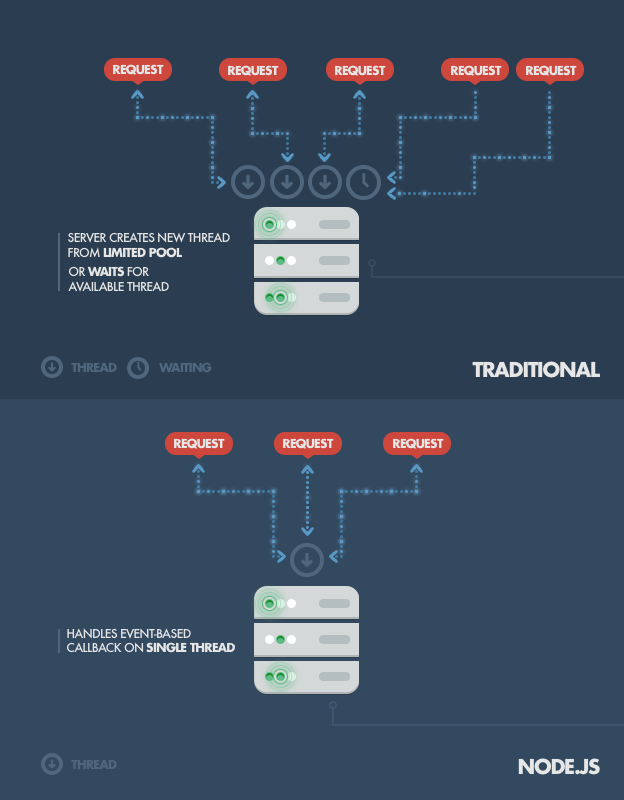
\includegraphics[width=0.5\textwidth]{figuras/cap2/diagram_traditional_vs_node_serverthread.png}
	\caption{Diagrama de \textit{Traditional} vs. Node.js \textit{server thread}}
\end{figure}



Un cálculo rápido: asumiendo que cada \textit{thread} potencialmente tiene asignado 2 MB de memoria con ella, corriendo en un sistema con 8 GB de RAM nos coloca en un teorico máximo de 4000 conexiones concurrentes, ademas del costo por cambio de contexto entre \textit{threads}. Ese es el escenario al con el cual tipicamente se encuentra en tecnicas tradicionales de \textit{web-serving}. Evitando todo eso, Node.js logra niveles de \textit{scalability} sobre 1M de conexciones concurrentes (como \textit{proof-of-concept}).
%A quick calculation: assuming that each thread potentially has an accompanying 2 MB of memory with it, running on a system with 8 GB of RAM puts us at a theoretical maximum of 4000 concurrent connections, plus the cost of context-switching between threads. That’s the scenario you typically deal with in traditional web-serving techniques. By avoiding all that, Node.js achieves scalability levels of over 1M concurrent connections (as a proof-of-concept).

Hay, porsupuesto, la cuestión de compartir un solo \textit{thread} entre todos los \textit{request} de clientes, y es una potencial trampa de escribir aplicaciones Node.js. Primeramente, \textit{heavy computation} puede asfixiar el unico \textit{thread} de Node.js y causan problemas en todos los clientes como \textit{incoming request} podrían ser bloqueados hasta que dicho \textit{computation} sea completado. En segundo lugar, desabolladores necesitan ser realmente cuidados en no permitir que una excepción \textit{bubbling up} al \textit{core} del \textit{event loop} de Node.js, el cual puede causar que la instancia Node.js termine (efectivamente \textit{crashing} el programa).
%There is, of course, the question of sharing a single thread between all clients requests, and it is a potential pitfall of writing Node.js applications. Firstly, heavy computation could choke up Node’s single thread and cause problems for all clients (more on this later) as incoming requests would be blocked until said computation was completed. Secondly, developers need to be really careful not to allow an exception bubbling up to the core (topmost) Node.js event loop, which will cause the Node.js instance to terminate (effectively crashing the program).

La técnica utilizada para evitar exepcines \textit{bubbling up to the surface} es pasando el error de regreso al \textit{caller} como parametro de \textit{callback} (en lugar de lanzarlos, como en otros ambientes). Incluso si alguna excepción no controlada conduzca a \textit{bubble up}, hay múltiples paradigmas y herramientas disponibles para monitorear el proceso Node y realizar lo necesario para recuperarse de un \textit{crashed instance} (aunque no este disponible para recuperar sesiones de usuarios), siendo el mas común el módulo Forever\cite{online_github_nodejitsu_forever}.
%The technique used to avoid exceptions bubbling up to the surface is passing errors back to the caller as callback parameters (instead of throwing them, like in other environments). Even if some unhandled exception manages to bubble up, there are mutiple paradigms and tools available to monitor the Node process and perform the necessary recovery of a crashed instance (although you won’t be able to recover users’ sessions), the most common being the Forever module, or a different approach with external system tools upstart and monit.

%NPM: The Node Package Manager

%When discussing Node.js, one thing that definitely should not be omitted is built-in support for package management using the NPM tool that comes by default with every Node.js installation. The idea of NPM modules is quite similar to that of Ruby Gems: a set of publicly available, reusable components, available through easy installation via an online repository, with version and dependency management.

%A full list of packaged modules can be found on the NPM website https://npmjs.org/ , or accessed using the NPM CLI tool that automatically gets installed with Node.js. The module ecosystem is open to all, and anyone can publish their own module that will be listed in the NPM repository. A brief introduction to NPM (a bit old, but still valid) can be found at http://howtonode.org/introduction-to-npm.

%Some of the most popular NPM modules today are:

%express - Express.js, a Sinatra-inspired web development framework for Node.js, and the de-facto standard for the majority of Node.js applications out there today.
%connect - Connect is an extensible HTTP server framework for Node.js, providing a collection of high performance “plugins” known as middleware; serves as a base foundation for Express.

%socket.io and sockjs - Server-side component of the two most common websockets components out there today.

%Jade - One of the popular templating engines, inspired by HAML, a default in Express.js.

%mongo and mongojs - MongoDB wrappers to provide the API for MongoDB object databases in Node.js.

%redis - Redis client library.
%coffee-script - CoffeeScript compiler that allows developers to write their Node.js programs using Coffee.
%underscore (lodash, lazy) - The most popular utility library in JavaScript, packaged to be used with Node.js, as well as its two counterparts, which promise better performance by taking a slightly different implementation approach.
%forever - Probably the most common utility for ensuring that a given node script runs continuously. Keeps your Node.js process up in production in the face of any unexpected failures.
%The list goes on. There are tons of really useful packages out there, available to all (no offense to those that I’ve omitted here).

%Examples of Where Node.js Should Be Used


%Where Node.js Can Be Used

%SERVER-SIDE WEB APPLICATIONS

%Node.js with Express.js can also be used to create classic web applications on the server-side. However, while possible, this request-response paradigm in which Node.js would be carrying around rendered HTML is not the most typical use-case. There are arguments to be made for and against this approach. Here are some facts to consider:

%Pros:

%If your application doesn’t have any CPU intensive computation, you can build it in Javascript top-to-bottom, even down to the database level if you use JSON storage Object DB like MongoDB. This eases development (including hiring) significantly.
%Crawlers receive a fully-rendered HTML response, which is far more SEO-friendly than, say, a Single Page Application or a websockets app run on top of Node.js.
%Cons:

%Any CPU intensive computation will block Node.js responsiveness, so a threaded platform is a better approach. Alternatively, you could try scaling out the computation [*].
%Using Node.js with a relational database is still quite a pain (see below for more detail). Do yourself a favour and pick up any other environment like Rails, Django, or ASP.Net MVC if you’re trying to perform relational operations.
%[*] An alternative to these CPU intensive computations is to create a highly scalable MQ-backed environment with back-end processing to keep Node as a front-facing ‘clerk’ to handle client requests asynchronously.
%Where Node.js Shouldn’t Be Used
%
%SERVER-SIDE WEB APPLICATION W/ A RELATIONAL DB BEHIND
%
%Comparing Node.js with Express.js against Ruby on Rails, for example, there is a clean decision in favour of the latter when it comes to relational data access.
%
%Relational DB tools for Node.js are still in their early stages; they’re rather immature and not as pleasant to work with. On the other hand, Rails automagically provides data access setup right out of the box together with DB schema migrations support tools and other Gems (pun intended). Rails and its peer frameworks have mature and proven Active Record or Data Mapper data access layer implementations, which you’ll sorely miss if you try to replicate them in pure JavaScript.[*]
%
%Still, if you’re really inclined to remain JS all-the-way (and ready to pull out some of your hair), keep an eye on Sequelize and Node ORM2—both are still immature, but they may eventually catch up.
%
%[*] It’s possible and not uncommon to use Node solely as a front-end, while keeping your Rails back-end and its easy-access to a relational DB.
%HEAVY SERVER-SIDE COMPUTATION/PROCESSING
%
%When it comes to heavy computation, Node.js is not the best platform around. No, you definitely don’t want to build a Fibonacci computation server in Node.js. In general, any CPU intensive operation annuls all the throughput benefits Node offers with its event-driven, non-blocking I/O model because any incoming requests will be blocked while the thread is occupied with your number-crunching.
%
%As stated previously, Node.js is single-threaded and uses only a single CPU core. When it comes to adding concurrency on a multi-core server, there is some work being done by the Node core team in the form of a cluster module [ref: http://nodejs.org/api/cluster.html]. You can also run several Node.js server instances pretty easily behind a reverse proxy via nginx.
%
%With clustering, you should still offload all heavy computation to background processes written in a more appropriate environment for that, and having them communicate via a message queue server like RabbitMQ.
%
%Even though your background processing might be run on the same server initially, such an approach has the potential for very high scalability. Those background processing services could be easily distributed out to separate worker servers without the need to configure the loads of front-facing web servers.
%
%Of course, you’d use the same approach on other platforms too, but with Node.js you get that high reqs/sec throughput we’ve talked about, as each request is a small task handled very quickly and efficiently.
%
%Conclusion
%
%We’ve discussed Node.js from theory to practice, beginning with its goals and ambitions, and ending with its sweet spots and pitfalls. When people run into problems with Node, it almost always boils down to the fact that blocking operations are the root of all evil—99% of Node misuses come as a direct consequence.
%
%In Node, blocking operations are the root of all evil—99% of Node misuses come as a direct consequence.
%
%Remember: Node.js was never created to solve the compute scaling problem. It was created to solve the I/O scaling problem, which it does really well.

%Why use Node.js? If your use case does not contain CPU intensive operations nor access any blocking resources, you can exploit the benefits of Node.js and enjoy fast and scalable network applications. Welcome to the real-time web.

\subsection{Desempeño de Node.js frente a sus competidores}
	A continuación se harán comparaciones en el desempeño de la plataforma  con algunos de sus símiles mas conocidos los cuales corresponden a:
	
	\begin{itemize}
		\item Java
		\item Ruby
		\item PHP
	\end{itemize}

\subsubsection{Node.js vs Java \cite{online_nodejs_paypal}}



La primera adopción que hizo Paypal con Node.js no fue una aplicación menor; esto fue su \textit{account overview page} y una de las mas \textit{trafficked} \textit{apps} en el \textit{website}. Ellos tomaron un gran riesgo, pero lo hicieron con la finalidad de determinar si realmente la nueva plataforma representaba una mejora con respecto al sistema actual.
%Our first adopter of node.js in production wasn’t a minor application; it was our account overview page and one of the most trafficked apps on the website. We decided to go big, but we also mitigated that risk by building the equivalent Java application in parallel. We knew how to deploy and scale Java applications, so if anything went wrong with the node.js app, we could fall back to the Java one. This provided the setting for some interesting data.

Una vez que la aplicación con Node.js logro las mismas funcionalidades que la aplicación actual, persivieron el siguiente resultado:

\begin{itemize}
\item Fue construida casi \textbf{el doble de rapido con menos personal}.
\item Escrito con un \textbf{33\% menos de lineas de código}.
\item Construida con \textbf{40\% menos de archivos}.
\end{itemize}

Por si solo, esto mostro evidencia que mostraba a los equipos desarrollar más rápido utilizando \textit{JavaScript}

Performance fue un tópico interesante. Se pudo analizar 2 aplicaciones con exactamente las mismas funcionalidades: una con \textit{framework} Java interno basado en Spring y la otra construida en \textit{kraken.js} usando \textit{express}, \textit{dust.js} y otros códigos \textit{open source}.
%Performance is a fun and debatable topic. In our case, we had two applications with the exact same functionality and built by roughly the same teams: one on our internal Java framework based on Spring and the other built on kraken.js using express, dust.js and other open source code.

Se ejecutaron los test adecuados utilizando \textit{hardware} de producción que probaran las rutas y recolectaran \textit{data} rendimiento y tiempo de respuesta.
%We ran our test suite using production hardware that tested the routes and collected data on throughput and response time.

\begin{figure}[h!]
	\centering
	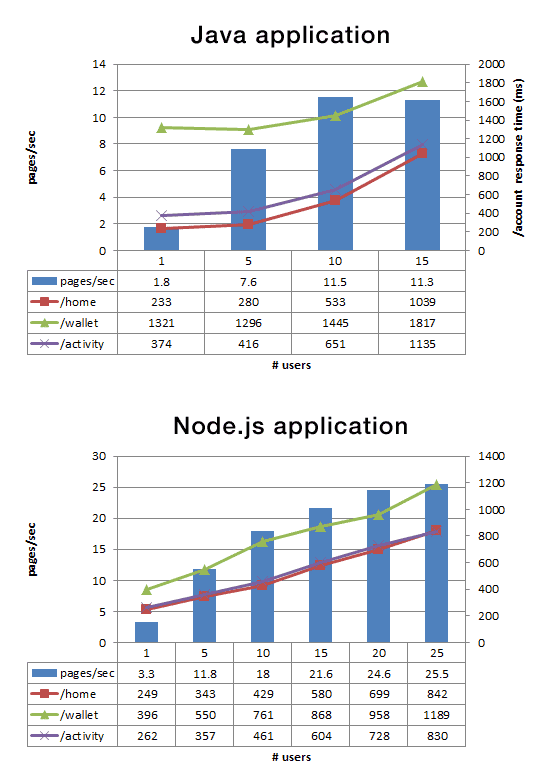
\includegraphics[width=0.6\textwidth]{figuras/cap2/java_nodejs_benchmark_paypal.png}
	\caption{\textit{Performance} de la aplicación en Java y Node.js}
	\label{cap2:figure:java_benchmark_paypal}
\end{figure}

Se observa que la aplicación que utiliza Node.js tiene:
%You can see that the node.js application had:



\begin{itemize}
\item El doble de solicitudes por segundo vs. la aplicación Java. Esto es incluso mas interesante porque los resultados iniciales de rendimiento estaban utilizando un solo núcleo para la aplicación Node.js, en comparación con cinco núcleos en Java. Se espere aumentar aun más esta brecha en el futuro.
%Double the requests per second vs. the Java application. This is even more interesting because our initial performance results were using a single core for the node.js application compared to five cores in Java. We expect to increase this divide further.
\item \textbf{Disminución en un 35\% en el tiempo promedio de respuesta} para la misma página. Esto se resulto ser \textbf{200ms mas rápido} en el servidor. Algo que los usuarios definitivamente notan.
%35% decrease in the average response time for the same page. This resulted in the pages being served 200ms faster— something users will definitely notice.
\end{itemize}


%There’s a disclaimer attached to this data: this is with our frameworks and two of our applications. It’s just about as apples-to-apples a performance test as we could get between technologies, but your milage may vary. That said, we’re excited by what we’ve seen from node.js’ raw performance.

Mas ejemplos de benchmark \cite{online_nodejs_java_dzone}


\subsubsection{Node.js vs PHP\cite{online_nodejs_php_loadimpact}}

No es justo comprar Node.js con PHP. Lo que realmente se compara es Node.js y PHP+Apacha2 ( u otro servidor http ). Es este caso particular, las pruebas fueron realizadas usando Apache2 y \textit{mod\_php}, dado que es por lejos la configuración mas común. 
%So no, it’s not fair to say that we compare Node.js and PHP. What we really compare is Node.js and PHP+Apache2 (or any other http server). For this article, I’ve used Apache2 and mod_php since it’s by far the most common configuration. Some might say that I’d get much better results if I had used Nginx or Lighthttpd as the http server for PHP. That’s most likely very true, but at the end of the day, server side PHP depends on running in multiple separate processes. Regardless if we create those processes with mod_php or fastcgi or any other mechanism. So, I’m sticking with the standard server setup for PHP and I think that makes good sense.





\begin{figure}[h!]
	\centering
	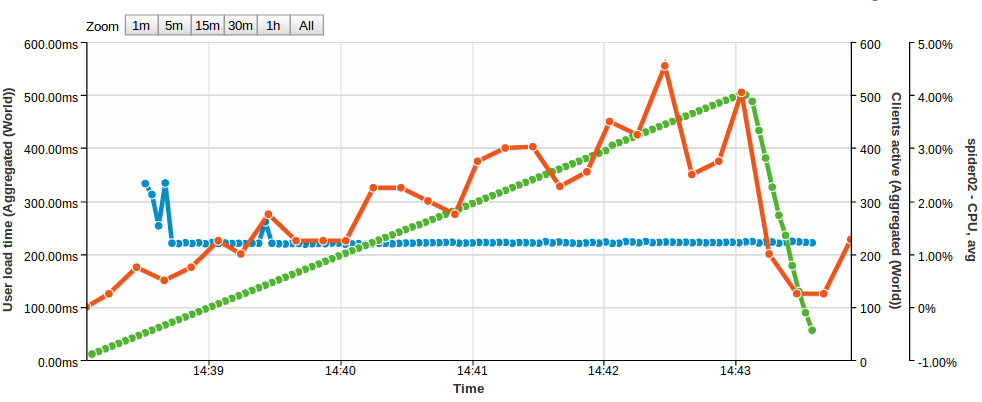
\includegraphics[width=0.6\textwidth]{figuras/cap2/node_benchmak_loadimpact.png}
	\caption{\textit{Performance} de la aplicación Node.js}
	\label{cap2:figure:java_benchmark_paypal}
\end{figure}

El primer gráfico muestra lo que sucede cuando se carga el test en el servidor utilizando Node.js. La respuesta de tiempo (azul) es mucho mas constante durante todo el test. 

%The first graph here shows what happens when we load test the Node.js server. The response time (blue) is pretty much constant all through the test. My back of a napkin analysis of the initial outliers is that they have to do with a cold MySQL cache. Now, have a look at the results from the PHP test:


\begin{figure}[h!]
	\centering
	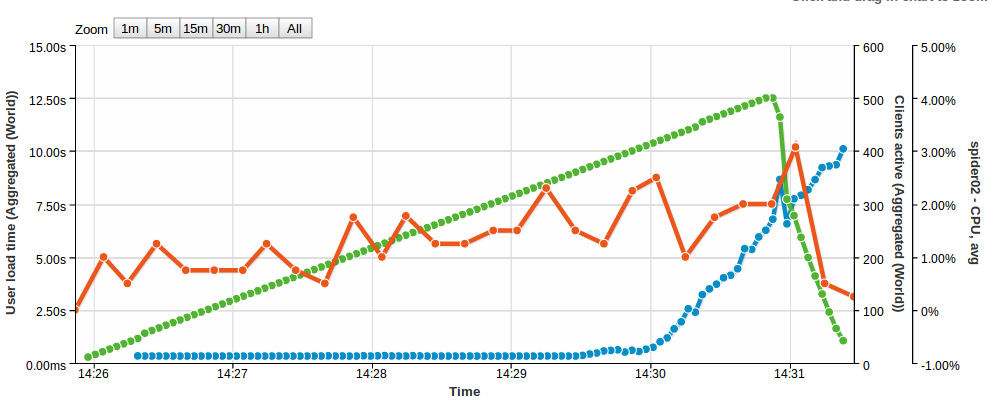
\includegraphics[width=0.6\textwidth]{figuras/cap2/phpapache_benchmak_loadimpact.png}
	\caption{\textit{Performance} de la aplicación en PHP/Apache}
	\label{cap2:figure:java_benchmark_paypal}
\end{figure}

Muy diferente los resultados para el caso de PHP. No es sencillo observar que sucede, pero las lineas azules están inicialmente estables a 320ms hasta cerca de 340 usuarios activos simultáneos. Después de eso, se observa un pequeño incremento en el tiempo de respuesta pero después de agregar mas usuarios activos simultáneos, el tiempo de respuesta se dispara por completo. 
%Quite different results. It’s not easy to see on this screen shot, but the blue lines is initially stable at 320 ms response time up to about 340 active concurrent users. After that, we first see a small increase in response time but after additional active concurrent users are added, the response time eventually goes through the roof completely.

¿ Qué problema tiene PHP/Apache?
%So what’s wrong with PHP/Apache?

La diferencia no es de sorprender. Esto es producto de la diferencia de arquitectura entre ambas soluciones.
%Ok, so what we’re looking at is not very surprising, it’s the difference in architecture between the two solutions. Let’s think about what goes on in each case.

Cuando Apache2 sirve a una pagina PHP, este deja la ejecución PHP a un \textit{child process} específico. Ese \textit{child process} puede solo manejar una solicitud PHP al mismo tiempo, así que si hay mas solicitudes, las otras deben esperar. En el servidor hay un máximo de 256 clientes (MaxClients) configurados vs 150 que vienen por defecto. Incluso si es posible aumentar el MaxClients hasta mas allá de 256, habrá problemas con la memoria interna(RAM), Al final, se necesita encontrar el balance correcto entre el máximo numero de solicitudes simultaneas y los recursos disponibles del servidor.
%When Apache2 serves up the PHP page it leaves the PHP execution to a specific child process. That child process can only handle one PHP request at a time so if there are more requests than than, the others have to wait. On this server, there’s a maximum of 256 clients (MaxClients) configured vs 150 that comes standard. Even if it’s possible to increase MaxClients to well beyond 256, that will in turn give you a problem with internal memory (RAM). At the end, you need to find the correct balance between max nr of concurrent requests and available server resources.

Pero para Node.js, es sencillo. Después de todo, cada solicitud es cerca de 30\% mas rápido que PHP, así que en \textit{performance}, el cual es una configuración extremadamente básica, Node.js es mas rápido. Ademas, en Node.js Todo esta en un solo proceso en el servidor. Un proceso manejando una solicitud activa. Así que no existe una comunicación interna de procesos entre diferentes instancias y el proceso madre. Incluso, pos solicitud, Node es mucho mas eficiente. PHP/Apache necesita muchísimo PHP y sobrecarga de procesos por cada simultaneo  \textit{worker/client}mientras Node compartirá la mayoría de su memoria entre las solicitudes.
%But for Node, it’s easier. First of all, in the calm territory, each request is about 30% faster than for PHP, so in pure performance in this extremely basic setup, Node is quicker. Also going for Node is the fact that everything is in one single process on the server. One process with one active request handling thread. So thre’s no inter process communication between different instances and the ‘mother’ process. Also, per request, Node is much more memory efficient. PHP/Apache needs to have a lot of php and process overhead per concurrent worker/client while Node will share most of it’s memory between the requests.

%Also note that in both these tests, CPU load was never a problem. Even if CPU loads varies with concurrent users in both tests it stays below 5% (and yes, I did not just rely on the graph, I checked it on the server as well). (I’ll write a follow up on this article at some point when I can include server memory usage as well). So we haven’t loaded this server into oblivion in any way, we’ve just loaded it hard enough for the PHP/Aapache architecture to start showing some of it’s problems.

Mas ejemplos de \textit{benchmark} \cite{online_nodejs_java_appdynamics}


%\subsubsection*{¿ Qué hace a Node.js mejor?}
%
%Node.js introduce al menos 2 nuevas características ( para una amplia audiencia ). Primero, la habilidad  de escribir código JavaScript en el lado del servidor. En teoría esto puede ser una ventaja dado que JavaScipt es mas importante que nunca en el lado del cliente y usando el mismo lenguaje en el servidor y en el navegador deberían haber muchísimos beneficios. 
%%Node.js introduces at least two new things (for a broader audience). First, the ability to write server side JavaScript code. In theory this could be an advantage since JavaScript is more important than ever on the client side and using the same language on server and browser would have many benefits. That’s at least quite cool.
%
%La otra cosa que introduce Node.js es que es completamente asíncrono y orientado al evento. Node.js esta basado en el supuesto que muchísimo código de computador realmente espera por I/O la mayoría del tiempo, como esperando por un archivo para ser escrito en el disco o por una solicitud MySQL para retornar \textit{data}. Para lograr eso, mas o menos cada función en Node.js es \textit{non-blocking}.
%%The other thing that makes Node.js different is that it’s completely asynchronous and event driven. Node is based on the realization that a lot of computer code actually just sits idle and wait for I/O most of the time, like waiting for a file to be written to disk or for a MySQL query to return data. To accomplish that, more or less every single function in Node.js is non-blocking.
%
%Cuando se solicita a nodo abrir un archivo, no se espera a que retorne. En lugar de eso, se le comunica a Node.js a que función se le entrega el resultado y continuar con otra ejecución. Esto conduce a una dramática diferencia  para estructurar el código con \textit{callback} anidados y funciones anónimas de clausura.  Terminaras con algo como esto:
%%When you ask for node to open a file, you don’t wait for it to return. Instead, you tell node what function to pass the results to and get on with executing other statements. This leads to a dramatically different way to structure your code with deeply nested callbacks and anonymous function and closures. You end up with something  like this:
%
%
%\medskip
%\begin{lstlisting}[caption= Ejemplo de anidación de funciones.]
%	doSomething(val, function(err,result){
%		doSomethingElse(result,function(err,res){
%			doAbra();
%			doKadabra(err, res, function() {
%				...
%				...
%			});
%		});
%	});
%\end{lstlisting}
%
%
%La cualidad que hace diferente a Node.js, es que no es necesario utilizar un servidor http(s) separado. Es completamente común poner Node.js detrás de un Nginx, pero eso no es estrictamente necesario. Así que el corazón de las aplicaciones \textit{web} típicas de Node.js  es la implementación de su servidor real.
%It’s quite easy to end up with very deep nesting that in my opinion sometimes affects code readability in a negative way. But compared to what gets said about PHP, that’s very mild critique. And.. oh! The third thing that is quite different is that in Node.js, you don’t have to use a separate http(s) server. It’s quite common to put Node.js behind a Nginx, but that’s not strictly needed. So the heart of a typical Node.js web application is the implementation of the actual web server.


*****************************************************************************


Hopefully, this shows the inherit differences in two different server technologies. One old trusted and one young and trending. Hopefully it’s apparent that your core technical choices will affect your server performance and in the end, how much load you can take. Designing for high load and high scalability begins early in the process, before the first line of code is ever written.

And sure, in real life, there are numerous of tricks available to reduce the effects seen here. In real life, lots of Facebook still runs on PHP.


\subsubsection{Node.js y \gloss{ecommerce}}

\gloss{ecommerce} es un excelente ejemplo de sistema que se puede ver totalmente beneficiado con el uso de Node.js en el \textit{server side}. 

\begin{itemize}
	\item \textbf{FRONT-END se movió desde el server-side al client-side( al menos en mobile )}. Una de las grandes consecuencias es que el server-side ya no es mas CPU Bound ahora es Memory Bound e I/O Bound. Node.js es \textit{event-driven}, lo cual implica eficiencia en I/O Bound y es extremadamente eficiente en el uso de memoria.
	\item Permite velocidad de desarrollo y ejecución. En otras palabras iteraciones rápidas.
	%Ease of Development-Some problem, somewhere has a solution best written in Brainf*ck. But implementing that solution (in Brainfuck) will be nearly impossible to write, let alone read. It will cost you time and a tremendous amount of effort. In general, you should use languages and platform that make development easier, not harder for you (or anyone that might work on it later).
	\item \textbf{Comunidad}: Existe una activa comunidad la cual esta constantemente solucionando dudas, ademas de proporcionar módulos para resolver problemas conocidos.
	\item \textbf{Reutilizar código}: \textit{Server-side} y \textit{client-side} usan el mismo lenguaje, permitiendo reutilización de componentes.
	\item \textbf{Optimiza el uso de recursos}: Los desarolladores de \textit{client-side} pueden desarrollar en \textit{server-side}, ya que son el mismo lenguaje.
	\item \textbf{Scalability}: Los sitions \textit{web} se encuentran en constante crecimiento. \textit{Scalability} es una consecuencia de la eficiencia que tiene Node.js para Memory Bound e I/O Bound
\end{itemize}

%+++++++++++++++++++++++++++++++++++++++++++++++++++++++++++++++++++++++
%
%
%Node no es la panacea para todo, tiene muchos issues con los cuales hay que lidiar, pero es probable una de las mejores soluciones que se pueden tomar(LinkedIn).
%
%***************************************************************************
%Kiran Prasad, Sr. Director, Mobile Engineering, LinkedIn
%
%Una pregunta interesante saber cuales son los problemas que te hicieron mirar hacia nodeJ(pregunta a KIRAN Prased)
%
%Cuando llegue a LinkedIN estabamos corriendo cosas en Ruby and Rails stack, una de las cosas que encontramos es que el FRONT-END se movio desde el server-side al client-side( al menos en mobile ). Ese gran shift cambio  las necesidades del front-end y el server-side.
%
%El server-side ya no es mas CPU Bound ahora es Memory Bound e I/O Bound
%
%Nodejs run de forma muy eficiente en I/O 
%
%Dio velocidad de desarrollo, de ejecución, iteraciónes mas rápidas 
%
%Este tipo de razones nos mostrarón la necesidad de I/O Bound necesitan ser I/O event
%Necesitaban eficiencia de memoria, y Node es super eficiente en ese sentido.
%La convinación de estos elementos  
%
%eficiencia en memoria
%
%
%
%***************************************************************************
%Sri Viswanath, SVP Engineering and Operations, Groupon
%
%
%
%Need low latency
%
%
%
%***************************************************************************
%Jigar Desai, Sr. Director, Platforms, eBay
%
%
%
%
%
%
%***************************************************************************
Billy Scott, PayPal

\section{\textit{Client side}}

Elegir el \textit{framework} correcto para un proyecto puede ternet un impacto tremendo en la habilida de entregar a tiempo y la habilidad para mantener el código en el futuro. ES ciertamente deseable un \textit{framework }solido, estable y provado, pero sin estar limitado por la opción. La \textit{web} estra evolucionando rapidamente; nuevas tecnologias surgen, y metodologias antiguas rapidamente se vuelven irrelebantes. Bajo este escenarió, se compararan 3 \textit{frameworks}
%In this article we are going to compare three popular MV* frameworks for the web: AngularJS vs. Backbone vs. Ember. Choosing the right framework for your project can have a huge impact on your ability to deliver on time, and your ability to maintain your code in the future. You probably want a solid, stable and proven framework to build upon, but don't want to be limited by your choice. The web is evolving fast — new technologies arise, and old methodologies quickly become irrelevant. Under this light, we are going to go through an in-depth comparison of the three frameworks.

\subsection{Meet The Frameworks}

%All the frameworks we are going to meet today have a lot in common: they are open-sourced, released under the permissive MIT license, and try to solve the problem of creating Single Page Web Applications using the MV* design pattern. They all have the concept of views, events, data models and routing. We are going to start with some quick background and history, and then dive in to compare the three frameworks.
%
%AngularJS was born in 2009 as a part of a larger commercial product, called GetAngular. Shortly after, Misko Hevery, one of the engineers who founded GetAngular, managed to recreate a web application that consisted of 17 thousand lines of code and took 6 months to develop in a mere 3 weeks using just GetAngular. Reducing the size of the application to just about 1,000 lines of code convinced Google to start sponsoring the project, turning it into the open-source AngularJS we know today. Amongst Angular's unique and innovative features are two-way data bindings, dependency injection, easy-to-test code and extending the HTML dialect by using directives.
%
%Backbone.js is a lightweight MVC framework. Born in 2010, it quickly grew popular as a lean alternative to heavy, full-featured MVC frameworks such as ExtJS. This resulted in many services adopting it, including Pinterest, Flixster, AirBNB and others.
%
%Ember's roots go way back to 2007. Starting its life as the SproutCore MVC framework, originally developed by SproutIt and later by Apple, it was forked in 2011 by Yehuda Katz, a core contributor to the popular jQuery and Ruby on Rails projects. Notable Ember users include Yahoo!, Groupon, and ZenDesk.

\subsection{Comunidad}

Una comunidad es uno de los factores mas importantes para considerar cuando se elije un \textit{framework}. Una extensa comunidad significa mas preguntas contestadas, mas modulos \textit{third-party}, mas tutoriales en youtube, etc. Angular es sin dudas la plataforma con mas apoyo  como se puede observar en \namref{tab:framework_community} \ref{tab:framework_community}.
%Community is one of the most important factors to consider when choosing a framework. A large community means more questions answered, more third-party modules, more YouTube tutorials…you get the point. I have put together a table with the numbers, as of August 16, 2014. Angular is definitely the winner here, being the 6th most-starred project on GitHub and having more questions on StackOverflow than Ember and Backbone combined, as you can see below:
%
%
\begin{table}[h!]
    \tiny
   
%\begin{tabular}{ |C{0.3\paperwidth}|C{0.3\paperwidth}| }
\begin{tabular}{ |L{0.1\paperwidth}|L{0.2\paperwidth}|L{0.2\paperwidth}|L{0.2\paperwidth}|}
\hline
	Metric&
	AngularJS &
	Backbone.js &
	Ember.js
	
\\ \hline
	Stars on Github&
	27.2k&
	18.8k&
	11k
\\ \hline
	Backbone.js&
	1.1.2&
	6.5kb&
	43.5kb (jQuery + Underscore) 20.6kb (Zepto + Underscore)
	
\\ \hline
	Third-Party Modules&
	800 ngmodules&
	236 backplugs&
	21 emberaddons
	
\\ \hline
	StackOverflow Questions&
	49.5k&
	15.9k&
	11.2k
	
\\ \hline
	YouTube Results&
	~75k&
	~16k&
	~6k
	
\\ \hline
	GitHub Contributors&
	928&
	230&
	393
	
\\ \hline
	Chrome Extension Users&
	150k&
	7k&
	38.3k
				
\\ \hline
\end{tabular}
    \caption{ Tamaño de la comunidad}
    \label{tab:framework_community}
\end{table}
%Metric	AngularJS	Backbone.js	Ember.js
%Stars on Github	27.2k	18.8k	11k
%Third-Party Modules	800 ngmodules	236 backplugs	21 emberaddons
%StackOverflow Questions	49.5k	15.9k	11.2k
%YouTube Results	~75k	~16k	~6k
%GitHub Contributors	928	230	393
%Chrome Extension Users	150k	7k	38.3k

%Todas las medidas, sin embargo, muestran simplemente el estado actual de cada \textit{framework}. También es interesante de observar cual \textit{framework} tienen el mayor crecimiento de popularidad. 
%All those metrics, however, merely show the current state of each framework. It is also interesting to see which framework has a faster-growing popularity. Fortunately, using Google Trends we can get an answer for that too:


\subsection{Framework Size}

El tiempo de carga para las paginas es crucial para el exito de un sitio \textit{web}. Los usuarios no muestran mucha paciencia cuando se trata de la velocidad de explorar; así que en muchos casos es deseado hacer todo lo posible para carga la aplicación tan rapido como sea posible. Hay 2 factores para observar que deben considerarse para el impacto del \textit{framework} en el tiempo de carga de la aplicación: el tamaño del \textit{framework} y el tiempo que le toma al \textit{framework} \textit{bootstrap}.
%Page load times are crucial for the success of your web site. Users do not exhibit much patience when it comes to the speed of browsing — so in many cases it is desired to do everything possible to make your application load as fast as possible. There are two factors to look at when considering the impact of the framework on the loading time of your application: framework size and the time it takes the framework to bootstrap.

Los \textit{assets} de JavaScript son usualmente 
%Javascript assets are usually served minified and gzipped, so we are going to compare the size of the minified-gzipped versions. However, merely looking at the framework is not enough. Backbone.js, despite being the smallest (only 6.5kb), requires both Underscore.js (5kb) and jQuery (32kb) or Zepto (9.1kb), and you will probably need to add some third party plug-ins to the mix.

\begin{table}[h!]
    \tiny
\begin{tabular}{ |L{0.1\paperwidth}|L{0.2\paperwidth}|L{0.2\paperwidth}|L{0.2\paperwidth}|}
\hline
	\textit{Framework}&
	Versión &
	Net Size &
	Size with required dependencies
	
\\ \hline
	AngularJS&
	1.2.22&
	39.5kb&
	39.5kb
\\ \hline
	Backbone.js&
	1.1.2&
	6.5kb&
	43.5kb (jQuery + Underscore) 20.6kb (Zepto + Underscore)
	
\\ \hline
	Ember.js&
	1.6.1&
	90kb&
	136.2kb (jQuery + Handlebars)
	
\\ \hline
\end{tabular}
    \caption{ Tamaño del \textit{framework}}
    \label{tab:framework_size}
\end{table}


\section{Full-Stack JavaScript}
%TODO

%Before digging into Node.js, you might want to read up on the benefits of using JavaScript across the stack which unifies the language and data format (JSON), allowing you to optimally reuse developer resources. As this is more a benefit of JavaScript than Node.js specifically, we won’t discuss it much here. But it’s a key advantage to incorporating Node in your stack.

%First of all, there are huge advantages to using a uniform language throughout your stack. My team uses a set of tools that we affectionately call the MEAN stack:­ MongoDB, ExpressJS, AngularJS, and Node.js. By coding with Javascript throughout, we are able to realize performance gains in both the software itself and in the productivity of our developers. With MongoDB, we can store our documents in a JSON-­like format, write JSON queries on our ExpressJS and NodeJS based server, and seamlessly pass JSON documents to our AngularJS frontend. Debugging and database administration become a lot easier when the objects stored in your database are essentially identical to the objects your client Javascript sees. Even better, somebody working on the client side can easily understand the server side code and database queries; using the same syntax and objects the whole way through frees you from having to consider multiple sets of language best practices and reduces the barrier to entry for understanding your codebase. This is especially important in a hackathon setting: the team may not have much experience working together, and with such little time to integrate all the pieces of your project, anything that makes the development process easier is gold.


\section{Resumen}
%TODO
Recapitulando, he demostrado que las soluciónes actuales de ecommerce pueden ser considerablemente mejoradas utilizando la tecnología actualmente presente. 
Importante notar que solo estoy ofreciendo una mejor solucuón a lo que ya existe, en ningun caso indico la solución que presento es la mejor posible. No se ha realizado un estudio sobre todas las opciones disponibles del mercado. Sin embargo esta solución ofrece

speed
scalability
flexibility
performance
